% !TeX source = ../main.tex

\chapter[Overview]{Overview}

\section{Notations on Sobolev spaces}
\label{sec:sobolev_notations}

\begin{figure}[!ht]
  \centering
  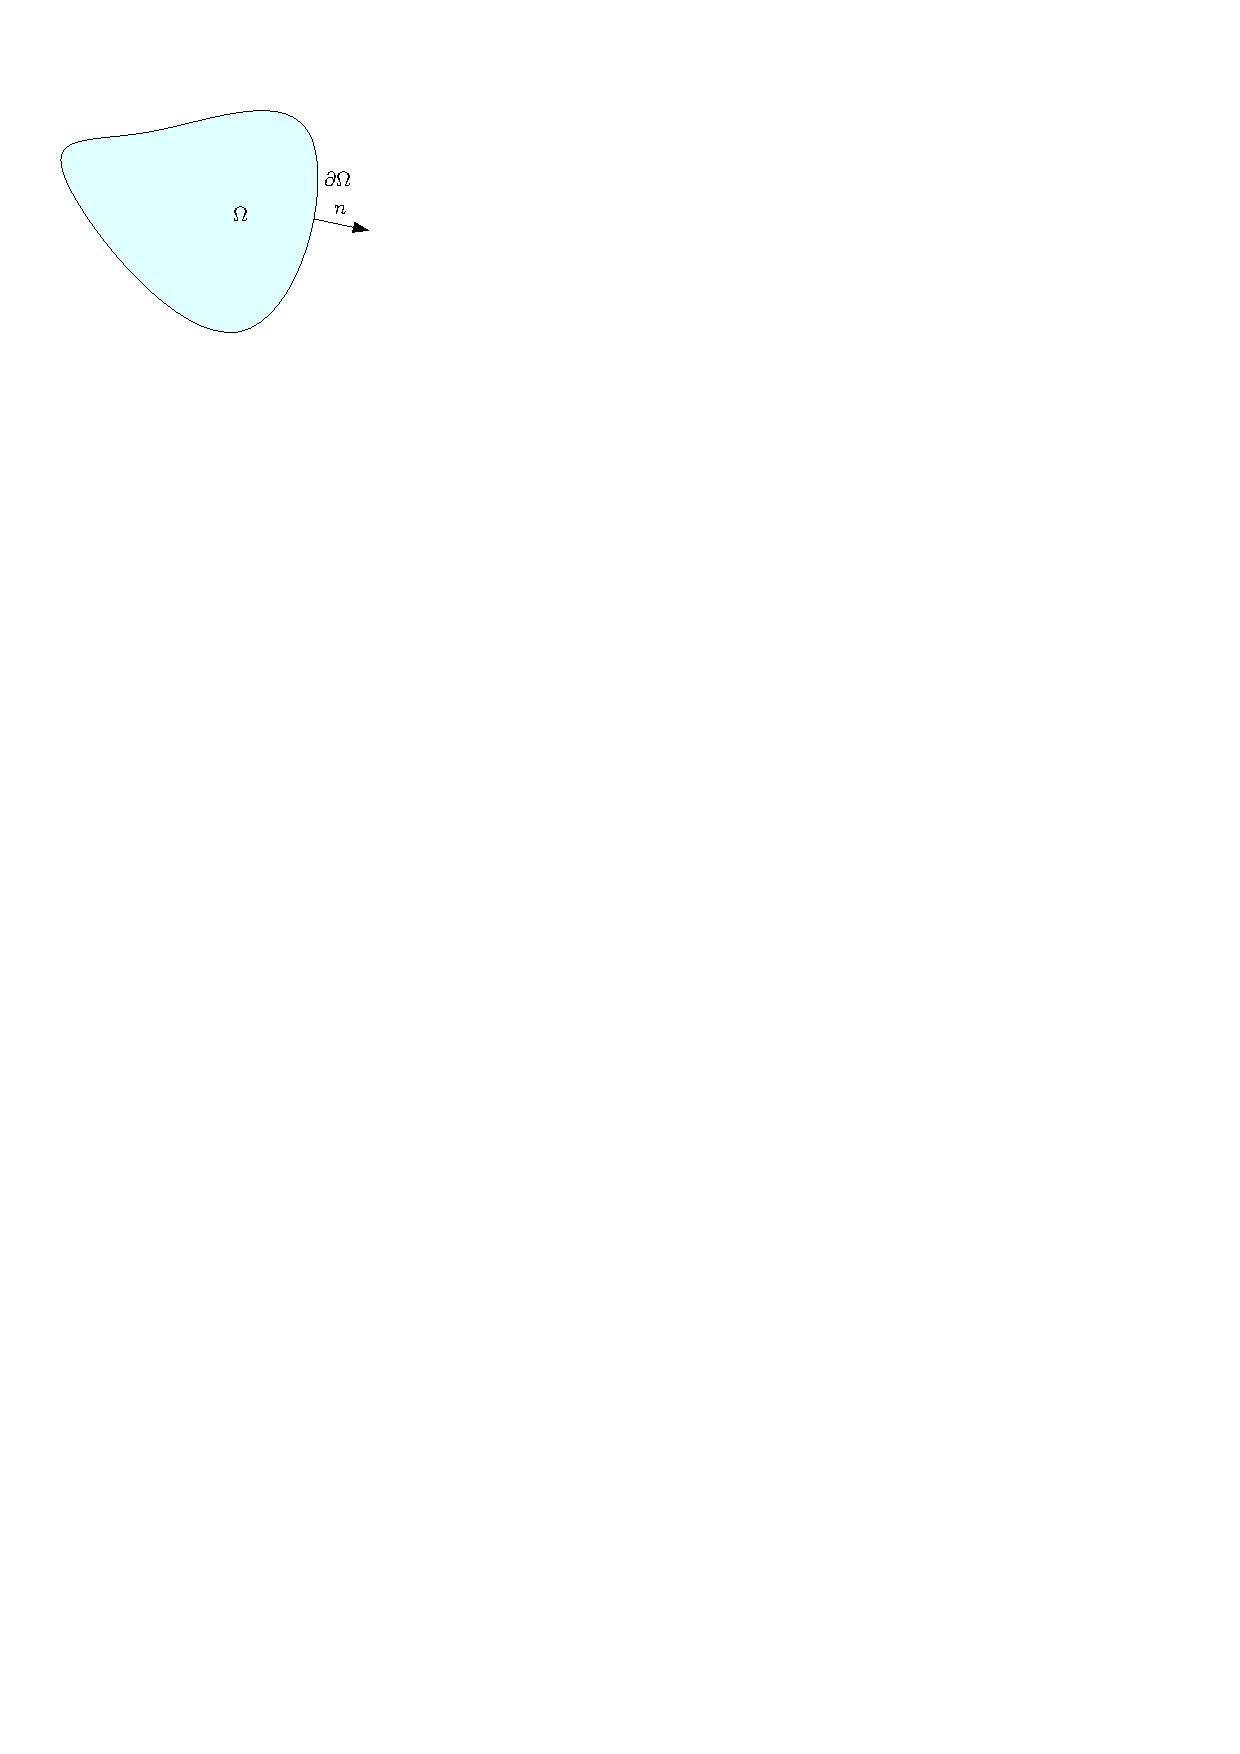
\includegraphics{domain}
  \caption{A Lipschitz domain $\Omega$ and its boundary $\partial\Omega$. We generally indicate with $n$ the outer normal to the boundary.}
  \label{fig:domain}
\end{figure}

Let $\Omega \subset \R^d$ be an open, bounded domain with Lipschitz boundary $\partial\Omega$. We begin by introducing some standard functional spaces that will be used throughout this course.

\subsection{Lebesgue spaces}

For $1 \leq p < \infty$, we define the Lebesgue space $L^p(\Omega)$ as the set of measurable functions $u: \Omega \to \R$ such that
\[
\|u\|_{L^p(\Omega)} := \left(\int_\Omega |u(x)|^p \diff x \right)^{1/p} < \infty.
\]

For $p = \infty$, we define $L^\infty(\Omega)$ as the space of essentially bounded measurable functions with the norm
\[
\|u\|_{L^\infty(\Omega)} := \operatorname{ess\,sup}_{x \in \Omega} |u(x)| < \infty.
\]

Finally we define the space of locally integrable functions as $L^1_{loc}(\Omega)$ where every function $u: \Omega \to \R$ is:
\begin{itemize}
\item measurable;
\item $u|_{K} \in L^1(K)$ for each compact subset $K \subseteq \Omega$.
\end{itemize}

These spaces, equipped with their respective norms, are Banach spaces. In particular, $L^2(\Omega)$ is a Hilbert space with the inner product
\[
(u, v)_{L^2(\Omega)} = \int_\Omega u(x) v(x) \diff x.
\]



\subsection{Weak derivatives}

Let $\alpha = (\alpha_1, \alpha_2, \ldots, \alpha_d)$ be a multi-index with $|\alpha| = \alpha_1 + \alpha_2 + \cdots + \alpha_d$. For a function $u \in C^{|\alpha|}(\Omega)$, we define the standard partial derivative
\[
D^\alpha u = \frac{\partial^{|\alpha|} u}{\partial x_1^{\alpha_1} \partial x_2^{\alpha_2} \cdots \partial x_d^{\alpha_d}}.
\]

For functions that are not sufficiently smooth, we introduce the concept of weak derivatives.

\begin{definition}[Weak derivative]
Let $u \in L^1_{\text{loc}}(\Omega)$ and $\alpha$ be a multi-index. A function $v \in L^1_{\text{loc}}(\Omega)$ is called the $\alpha$-th weak derivative of $u$, denoted by $D^\alpha u = v$, if
\[
  \int_\Omega v(x) \phi(x) \diff x =  (-1)^{|\alpha|} \int_\Omega u(x) D^\alpha \phi(x) \diff x  \quad \forall \phi \in C_0^\infty(\Omega).
\]
\end{definition}

\subsection{Sobolev spaces $W^{k,p}(\Omega)$ and $H^k(\Omega)$}

For integers $k \geq 0$ and $1 \leq p \leq \infty$, we define the Sobolev space $W^{k,p}(\Omega)$ as
\[
W^{k,p}(\Omega) = \{u \in L^p(\Omega) : D^\alpha u \in L^p(\Omega) \text{ for all } |\alpha| \leq k\},
\]
where $D^\alpha u$ are weak derivatives. For $p < \infty$, this space is equipped with the norm
\[
\|u\|_{k,p,\Omega} := \left( \sum_{|\alpha| \leq k} \|D^\alpha u\|_{L^p(\Omega)}^p \right)^{1/p}.
\]

For $p = \infty$, we define
\[
\|u\|_{k,\infty,\Omega} = \max_{|\alpha| \leq k} \|D^\alpha u\|_{L^\infty(\Omega)}.
\]

We also define the seminorm
\[
|u|_{k,p,\Omega} = \left( \sum_{|\alpha| = k} \|D^\alpha u\|_{L^p(\Omega)}^p \right)^{1/p},
\]
with a similar modification for $p = \infty$.

When $p = 2$, we denote $W^{k,2}(\Omega)$ by $H^k(\Omega)$, which is a Hilbert space with the inner product
\[
(u, v)_{H^k(\Omega)} = \sum_{|\alpha| \leq k} (D^\alpha u, D^\alpha v)_{L^2(\Omega)}.
\]

In this case, we simplify the notation for the definition of the norm, and we omit the subscript $2$ (and the domain $\Omega$ if no confusion can arise) for the $H^k$-norm:
\[
  \|u\|_{k} \equiv \|u\|_{k,\Omega} := \|u\|_{k,2,\Omega} = \left( \sum_{|\alpha| \leq k} \|D^\alpha u\|_{L^2}^2 \right)^{1/2}.
\]

\subsection{Sobolev spaces with vanishing boundary values}

For functions in Sobolev spaces, we define the subspace of functions vanishing on the boundary $\partial\Omega$. For $1 \leq p < \infty$, we define
\[
W_0^{k,p}(\Omega) = \overline{C_0^\infty(\Omega)}^{\|\cdot\|_{W^{k,p}(\Omega)}},
\]
that is, the closure of $C_0^\infty(\Omega)$ with respect to the $W^{k,p}$-norm.

In particular, we denote $W_0^{k,2}(\Omega)$ by $H_0^k(\Omega)$. A key property of $H_0^1(\Omega)$ is the Poincaré inequality, which states that there exists a constant $C_{\Omega} > 0$ such that
\[
\|u\|_{L^2(\Omega)} \leq C_{\Omega} \|\nabla u\|_{L^2(\Omega)} \quad \forall u \in H_0^1(\Omega).
\]

This implies that the seminorm $|u|_{H^1(\Omega)} = \|\nabla u\|_{L^2(\Omega)}$ is actually a norm on $H_0^1(\Omega)$ equivalent to the standard $H^1$-norm.

\subsection{Dual spaces}

For a Banach space $X$, we denote by $X'$ its dual space, i.e., the space of continuous linear functionals on $X$. For example, $H^{-1}(\Omega) = (H_0^1(\Omega))'$ denotes the dual of $H_0^1(\Omega)$. We indicate with $\langle \cdot, \cdot \rangle$ the duality pairing between $X$ and $X'$, and we write $f(u) \equiv \langle f, u \rangle$ for $f \in X'$ and $u \in X$.

The norm of a functional $f \in X'$ is defined as
\[
\|f\|_{X'} = \sup_{u \in X} \frac{|\langle f, u \rangle|}{\|u\|_X}.
\]

\subsection{Riesz representation theorem}

For Hilbert spaces, we have a powerful characterization of the dual space through the Riesz representation theorem.

\begin{theorem}[Riesz representation theorem]
  \label{theo:riesz_representation}
Let $H$ be a Hilbert space with inner product $(\cdot, \cdot)_H$. For every bounded linear functional $f \in H'$, there exists a unique element $\tau f \in H$ such that
\[
f(v) = \langle f, v \rangle = (\tau f, v)_H \quad \forall v \in H,
\]
and furthermore,
\[
\|f\|_{H'} = \|\tau f\|_H.
\]
The operator $\tau$ is the so called Riesz operator.
\end{theorem}

This theorem establishes an isometric isomorphism between a Hilbert space and its dual. In particular, for $H = L^2(\Omega)$, given $f \in L^2(\Omega)$, we can identify the functional 
\[
v \mapsto \int_\Omega f v \, \mathrm{d}x
\]
with $f$ itself. Similarly, for $H = H^1_0(\Omega)$, every element in $H'$ can be represented uniquely as an inner product with some element in $H$.

The Riesz representation theorem is especially useful in characterizing the action of operators and in proving existence of solutions to variational problems, as it allows us to convert abstract duality pairings into concrete inner products.

\subsection{Bilinear forms and operators}

Let $X$ and $Y$ be Banach spaces. A bilinear form $a: X \times Y \to \mathbb{R}$ is said to be bounded (or continuous) if there exists a constant $C > 0$ such that
\[
|a(u, v)| \leq C \|u\|_X \|v\|_Y \quad \forall u \in X, \forall v \in Y.
\]

Given a bilinear form $a: X \times Y \to \mathbb{R}$, we can define its associated operator $A: X \to Y'$ by
\[
\langle Au, v \rangle = a(u, v) \quad \forall u \in X, \forall v \in Y,
\]
where $\langle \cdot, \cdot \rangle$ denotes the duality pairing between $Y'$ and $Y$.

The operator $A$ is linear and it inherits the boundedness of $a$, i.e.,
\[ 
  \|A\|_* := \|A\|_{\mathcal{L}(X,Y')} = \sup\limits_{u \in X, v \in Y} \frac{|a(u,v)|}{\|u\|_X \|v\|_Y}.
\]

When $X = Y$ is a Hilbert space, a bilinear form $a: X \times X \to \mathbb{R}$ is said to be:
\begin{itemize}
  \item Symmetric if $a(u, v) = a(v, u)$ for all $u, v \in X$
  \item Coercive (or elliptic) if there exists $\alpha > 0$ such that $a(u, u) \geq \alpha \|u\|_X^2$ for all $u \in X$
\end{itemize}

\subsection{Trace spaces and the trace operator}

For functions in $H^1(\Omega),$ we can define their traces on the boundary $\partial\Omega$. The trace operator 
\[
\gamma: H^1(\Omega) \to H^{1/2}(\partial\Omega)
\]
is a bounded linear operator that extends the classical restriction to the boundary. For simplicity, we often write $u|_{\partial\Omega}$ for $\gamma(u)$.

The space $H^{1/2}(\partial\Omega)$ is a fractional Sobolev space on the boundary, and it can be characterized as the set of traces of $H^1(\Omega)$ functions.

A fundamental result is that $u \in H_0^1(\Omega)$ if and only if $u \in H^1(\Omega)$ and $\gamma(u) = 0$.

\subsection{Sobolev embeddings}

Sobolev spaces embed into other spaces in ways that formalize the intuitive notion that functions with more derivatives tend to be more regular. The Sobolev embedding theorems are crucial tools that allow us to relate Sobolev spaces to classical function spaces.

\begin{theorem}[Sobolev embedding]
Let $\Omega \subset \mathbb{R}^d$ be a bounded domain with Lipschitz boundary, $k \geq 0$ an integer, and $1 \leq p < \infty$. Then:

\begin{enumerate}
  \item If $kp > d$, then the following continuous embedding holds:
  \[
  W^{k,p}(\Omega) \hookrightarrow C^{0}(\overline{\Omega}),
  \]
  i.e., every function in $W^{k,p}(\Omega)$ has a continuous representative.
  
  \item If $s \geq 1$, $p,q \in [1, \infty]$, and 
  \[
  s - \frac{d}{p} > k - \frac{d}{q},
  \]
  then the following continous inclusion holds true:
  \[ 
    W^{s,p}(\Omega) \subset W^{t,q}(\Omega).
  \]
\end{enumerate}
\end{theorem}

The first case is of particular interest when we need our functions to be continuous. The condition $kp > d$ gives us a relationship between:

\begin{itemize}
  \item The order of derivatives $k$
  \item The integrability $p$ of those derivatives
  \item The dimension $d$ of the domain
\end{itemize}

For example, in two dimensions ($d=2$):
\begin{itemize}
  \item $H^2(\Omega) = W^{2,2}(\Omega) \hookrightarrow C^0(\overline{\Omega})$ since $2 \cdot 2 > 2$
  \item $W^{1,p}(\Omega) \hookrightarrow C^0(\overline{\Omega})$ for any $p > 2$
  \item $H^{1}(\Omega) \not\hookrightarrow C^0(\overline{\Omega})$.
\end{itemize}

More generally, in $d$ dimensions, we need $k > \frac{d}{p}$ to ensure continuity.

These embedding results are particularly important in numerical analysis, as they help determine when finite element approximations lead to continuous functions. For standard Lagrangian finite elements, the continuity of basis functions is essential, and these embedding theorems provide the theoretical foundation for when such continuity can be expected.

%****************************************************************
% Lezione 27 febbraio
%****************************************************************

\section{Model problem: the Poisson equation}

Let $\Omega$ be an open, bounded, Lipschitz subset of $\R^d$. Let also $\partial\Omega$ be its boundary.
Consider the following Poisson problem:
\[
\begin{cases} \marginpar{Strong formulation}
-\Delta u = f \qquad &\text{in $\Omega$} \\
u =  0 \qquad &\text{on $\partial \Omega$}
\end{cases}
\]
where, as usual,
\[
\Delta = \sum_{i=1}^d \frac{\partial^2}{\partial x_i^2}.
\]
If we want to find a numerical solution for this problem, two approaches can be followed:
\begin{itemize}
\item discretize $-\Delta$ (\emph{finite differences});
\item consider the \emph{weak formulation} of the problem (\emph{finite elements}).
\end{itemize}

Finite differences work well if $\Omega$ is a rectangular or parallelepiped domain (e.g. a square, a cube and so on) and if $f$ is regular enough (e.g. continuous). In applications, however, the domain's boundary may not be nice at all, and $f$ may not even be continuous.
The finite element approach tries to overcome these difficulties, by shifting the problem to finding a good finite dimensional space that approximates the functional space where the exact solution lives.

The advantage, when compared to, e.g., finite differences, is that we don't discretize the differential operator -- which maintains its continuous definition --  but instead we restrict our exploration of candidate solutions to simple spaces (i.e., space of piecewise polynomial functions), for which we can easily compute the action of the differential operator in an exact way.

To make a concrete example, let us consider the Poisson problem, and let's derive its weak formulation.
Let $\phi \in \D$ a test function (usually $\D=C_0^\infty(\Omega)$). We multiply by $\phi$ both sides of the PDE in the strong formulation and then integrate:
\[
\int_\Omega -\Delta u \phi = \int_\Omega f \phi.
\]
If we integrate by parts and use the fact that $\restr{u}{\partial \Omega} = \restr{\phi}{\partial\Omega} = 0$, we get:
\[
\int_\Omega \nabla u \nabla \phi = \int_\Omega f \phi.
\]
More in general, if we replace $\D$ with some appropriate function space $V$, the weak formulation will be: given $f\in V'$, find $u\in V$ such that
\begin{equation} \label{eqn:weak_1} \marginpar{Weak form (1)}
\int_\Omega \nabla u \nabla v = \int_\Omega f v \quad \forall v\in V.
\end{equation}
with the agreement that, being $f \in V'$, the RHS is in fact a duality.

On one side, we need that $\int_\Omega | \nabla u \nabla v | < +\infty$, and on the other side, we need that $u$ and $v$ should be zero on the domain boundary. A natural choice is then the Hilbert space $H^1_0(\Omega)$.

How do we guarantee that a solution to such problem exists? We prove this in an abstract Hilbert setting:
\begin{lemma}[Lax-Milgram]\label{lemma:lax-milgram}\marginpar{Lax-Milgram lemma}
Let $V$ be a Hilbert space and let $a: V\times V \to \R$ be a bilinear operator such that:
\begin{itemize}
\item $a$ is \emph{bounded}, i.e. $\exists c>0$ s.t. 
\[
 a(u,v) \le c \norm{u}_V \norm{v}_V \qquad \forall u,v \in V
 \] 
 (sometimes, we refer to the constant $c$ as $\norm{A}_*$);
\item $a$ is \emph{coercive}, i.e. $\exists \alpha >0$ s.t. 
\[
  a(u,u) \ge \alpha \norm{u}_V^2 \qquad \forall u \in V.
\]
\end{itemize}
Then, given $f\in V'$, the following problem
\begin{equation}\label{eqn:weak_laxmilgram}
a(u,v) = \langle f,v \rangle \quad \forall v\in V
\end{equation}
admits a unique solution $u_0$. Moreover, $u_0$ satisfies the following inequality:
\[
\norm{u_0}_V \le \frac{\norm{f}_{V'}}{\alpha}.
\]
\end{lemma}
\begin{proof}
  Let's consider the linear operator $A: V \to V'$ defined by $A(u) = a(u,\cdot)$.
  Boundedness of $a$ implies that $A$ is a bounded operator, and coercivity implies that 
  \[
    \langle A u, u \rangle = a(u,u) \ge \alpha \norm{u}_V^2 \quad \forall u \in V.
  \]
  
  Let us consider the map $\phi: V \mapsto V$ defined by 
  \[ 
    \phi(v) = v - \rho \tau(A v - f),
  \]
  where $\rho$ is a positive constant to be chosen later, and $\tau$ is the Riesz operator defined in Theorem~\ref{theo:riesz_representation}. By construction, if $u$ is a fixed point of $\phi$, i.e., $u= \phi(u)$, then $u$ necessarily satisfies $A u = f$. Conversely, if $u$ satisfies $Au=f$, then $u$ is also a fixed point of $\phi(u)=u$. 
  
  We want to show that ellipticity is enough to guarantee that there exists a $\rho$ such that $\phi$ is a contraction, i.e., $\exists! ~u$ s.t. $Au=f$.
  
  We have:
  \begin{align*}
    \norm{\phi(u) - \phi(v)}_V^2 & = \norm{u - v - \rho \tau(A(u - v))}_V^2 \\
    & = \norm{u - v}_V^2 - 2 \rho \langle A(u - v), u - v \rangle + \rho^2 \norm{A(u - v)}_{V'}^2 \\
    & \leq \norm{u - v}_V^2 - 2 \rho \alpha \norm{u - v}^2_V + \rho^2 \|A\|^2 \norm{u - v}_V^2 \\
    & \leq  (1 - 2\rho \alpha + \rho^2 \|A\|^2) \norm{u - v}_V^2.
  \end{align*}
  By choosing $\rho$ such that $0<1 - 2\rho \alpha + \rho^2 \|A\|^2 < 1$, (i.e., $\rho<\frac{2\alpha}{\|A\|}$) we have that $\phi$ is a contraction, and by the Banach fixed point theorem, we have that there exists a unique fixed point $u$ of $\phi$, which is the solution of the problem.
  
  Finally, we can estimate the norm of $u$ by the norm of $f$ and the coercivity constant $\alpha$:
  \[
  \alpha \norm{u}_V^2 \leq \langle A u, u \rangle = \langle f, u \rangle \leq \norm{f}_{V'} \norm{u}_V \qquad \Longrightarrow \qquad \norm{u}_V \leq \frac{\norm{f}_{V'}}{\alpha}.
  \]
\end{proof}

In the Poisson problem's case, the bilinear operator is
\[
a(u,v) = \int_\Omega \nabla u \nabla v,
\]
which is clearly bounded and coercive if $V=H_0^1(\Omega)$. In particular, coercivity follows from the Poincaré inequality which implies that the norm in $V$ is equivalent to the $H^1$ seminorm
\[
\abs{u}_{1,2} = \norm{\nabla u}_{L^2}.
\]
Hence, the weak formulation of the Poisson problem admits a unique solution by the Lax-Milgram lemma.

\section{Introduction to finite elements method}

The reason why the finite element method is powerful is that the differential operators stay untouched and, instead, what is to be simplified is \emph{the set in which the solutions live}. We construct a sequence of subspaces $V_h \subset V$ such that $V_h = \Span\{v_i\}_{i=1}^n$, with $n$ depending on $h$. Then we restrict the weak problem to $V_h$, which inherits the norm from $V$: given $f \in V'$, find $u_h \in V_h$ s.t.
\begin{equation} \label{eqn:weak_2} \marginpar{Discrete weak form}
a(u_h,v_h) = \langle f,v_h \rangle \quad \forall v_h\in V_h.
\end{equation}
The element $u_h$ will be our candidate approximate solution. Since $V_h$ is a Hilbert space, and the bilinear operator $a(\cdot, \cdot)$ is coercive in the entire $V$, then also Problem~\eqref{eqn:weak_2} satisfies the hypotheses of Lax-Milgram lemma, and we conclude that there exists a unique solution. For completeness, however, we shall  prove its existence also using Ritz method.

Since $u_h \in V_h$, there exist unique coefficients $\{u^j\}_{j=1}^n$ such that
\[
u_h = \sum_{j} u^j v_j.
\]
The weak problem \ref{eqn:weak_2} then becomes:
\[
a\left(\sum_{j} u^j v_j ,v_h\right) = \langle f,v_h \rangle \quad \forall v_h\in V_h.
\]
In particular, it will suffice for us to check it for a basis of $V_h$:
\[
\sum_{j} a(v_j, v_i)  u^j = \langle v_i,f \rangle \quad \forall i=1,\dots,n.
\]
Here we have rearranged the objects in the brackets and used linearity to make it clearer that this is a matrix identity: if $A$ is the matrix whose entries are $A_{ij}=a(v_j, v_i)$, then we have to solve the linear system
\[
A \mathbf{u} = \mathbf{f}
\]
where $\mathbf{u}=\{u^i\}_{i=1}^n$ and $\mathbf{f}=\{\langle f, v_i\rangle\}_{i=1}^n$.
In particular, $A$ is clearly symmetric and positive definite due to the coercivity of $a$:
\[
\mathbf{u}^T A \mathbf{u} = a(\sum_{i} u^i v_i, \sum_{j} u^j v_j) \ge \alpha \norm{\sum_{i} u^i v_i}^2 \ge 0
\]
and this, by linearity, is zero if and only if every $u^i$ is zero. We conclude that $A$ is non singular, hence $u_h$ exists and is unique.

We now seek a way to control \emph{a priori} the error introduced by the restriction to $V_h$.
\begin{lemma}[Ceà]\marginpar{Ceà's lemma} \label{lemma:cea}
In the setting of the Lax-Milgram lemma, let $u\in V$ be the solution of the weak problem~\eqref{eqn:weak_laxmilgram} and $u_h \in V_h$ a solution of~\eqref{eqn:weak_2}. Then:
\[
\norm{u - u_h} \le \frac{\norm{A}}{\alpha} \inf_{v_h \in V_h} \norm{u - v_h}.
\]
\end{lemma}
\begin{proof}
Observe that, since $u$ solves the weak problem in the whole $V$, then also
\[
a(u,v_h) = \langle f,v_h \rangle \quad \forall v_h\in V_h.
\]
By linearity, it follows that
\[
a(u - u_h,v_h) = 0 \quad \forall v_h\in V_h.
\]
In particular, this is also true if we substitute $v_h$ with $v_h - u_h$, which is still in $V_h$:
\[
a(u - u_h, v_h - u_h) = 0 \quad \forall v_h\in V_h.
\]
This is an orthogonality property of the error. Now we exploit the properties of $a$:
\begin{align}
\alpha \norm{u - u_h}^2 & \le a(u - u_h, u - u_h) \\
& = a(u - u_h, u - v_h) + a(u - u_h, v_h - u_h) \\
& = a(u - u_h, u - v_h) \\
& \le \norm{A} ~\norm {u - u_h} ~ \norm {u - v_h} \quad \forall v_h \in V_h.
\end{align}
The thesis follows by simplifying $\norm{u - u_h}$ on both sides of the inequality, and taking the infimum over $v_h \in V_h$.
\end{proof}

The meaning of Ceà's Lemma is: it suffices to control the error only in $V_h$ in order to have a good approximation of $u$. This is a step in the right direction, because in practice the functions in $V_h$ will be piecewise polynomials, hence their derivatives will be well defined and we won't need to approximate them. However, there are still some problems left:
\begin{itemize}
\item How do we approximate an arbitrary domain $\Omega$?
\item How do we approximate $V$ with $V_h$? Meaning, we seek to construct $V_h$ in such a way that $\text{dist}(V,V_h) = c h^k$ for some $k$, where
\[
\text{dist}(V,V_h) = \sup_{u\in V} \inf_{v_h \in V_h} \norm{u - v_h}.
\]
\item In practice, $u$ is unknown, but the RHS of the error estimate contains $u$. How do we manage this?
\end{itemize}

To approximate an arbitrary domain $\Omega$, we typically employ a process called mesh generation:

\begin{itemize}
  \item We partition the domain $\Omega$ into a collection of simple geometric shapes called elements (triangles/tetrahedra or quadrilaterals/hexahedra).
  \item This collection $\mathcal{T}_h = \{K_1, K_2, \ldots, K_M\}$ forms a triangulation or mesh of $\Omega$.
  \item The parameter $h$ represents the maximum diameter of any element in the mesh.
  \item For domains with curved boundaries, we often use:
  \begin{itemize}
    \item Piecewise linear/polynomial approximation of the boundary
    \item Isoparametric elements where the same shape functions describe both the geometry and solution
  \end{itemize}
\end{itemize}

The second problem is solved by using a \emph{finite element space} $V_h$ that is \emph{locally} defined on the elements of the mesh. The idea is to construct a finite dimensional space $V_h$ such that:
\begin{itemize}
  \item The functions in $V_h$ are piecewise polynomials defined on the elements of the mesh;
  \item Globally, the functions in $V_h$ are also members of the continuous space $V$ (i.e., the approximation is conforming, or $V_h \subseteq V$);
  \item The dimension of $V_h$ grows with the number of elements in the mesh, and the approximation improves as the mesh is refined (i.e., as $h$ decreases);
  \item The functions (and their derivatives) in $V_h$ can be easily evaluated and manipulated.
\end{itemize}

\section{An example: the 1-dimensional case}

Let $\Omega = (a,b)$. In order to discretize it, we consider a set of $n+2$ points $\Set{x_i}_{i=0}^{n+1}$ such that
\[
a = x_0 < x_1 < \dots < x_{n+1} = b.
\]
To keep things simple, let
\[
x_i = a+ih, \quad h = \frac{b-a}{n+1}.
\]
Let $V=H_0^1((a,b))$. Now consider
\[
V_h = \Set{v \in C^0([a,b]): \restr{v}{[x_i, x_{i+1}]}\in \P^1([x_i, x_{i+1}]) \,\forall i=0,\dots,n, \, v(a)=v(b)=0}
\]
where $\P^1$ denotes the space of polynomials of degree at most 1. This space has dimension $n$ and contains piecewise linear functions on $[a,b]$ which are zero on the boundary.

We proceed to find a basis for it: let $v^i(u) := u(x_i)$ the evaluation of $u$ in the node $x_i$, for $i=1,\dots,n$. If $u$ were in $\D$, then $v^i$ would act as a Dirac delta $\delta(x-x_i)$, since
\[
\langle v^i, u \rangle = \int_\Omega \delta(x-x_i) u(x) \diff x = u(x_i).
\]
We construct functions $v_j \in V_h$ such that
\[
v^i(v_j) = \delta_{ij} = \begin{cases}
1 \quad \text{if } i=j \\
0 \quad \text{if } i\ne j
\end{cases}
\quad \forall i,j \in \{1,\dots,n\}.
\]
In practice, for every node $x_j$ in the interior of $[a,b]$ we are considering a piecewise linear function that is one on that node and zero on any other node. It is clear that the functions $\{v_j\}_{j=1}^{n}$\footnote{These functions are also called "Hat functions" for their peculiar hat form.} form a basis for the space $V_h$. These are the so-called \emph{shape functions}. Instead, the $v^i$-s form a basis for $V_h'$ and are called the \emph{nodal basis functions}.

Let us now get back to the Poisson problem. In the 1-dimensional case, the entries of the matrix $A$ are of the form
\[
A_{ij} = \int_a^b v_j'(x) v_i'(x) \diff x.
\]
Since the nodal functions have been constructed in a \emph{localized} way, it is immediate to notice that $A_{ij} = 0$ whenever the supports of the involved nodal functions do not intersect. This is a distinguishing feature of a finite element method: the matrix $A$ is constructed in a way that makes it \emph{sparse}. In particular, in this case we have
\[
A_{ij} = \begin{cases}
0 \quad &\text{if } \abs{i-j}>1 \\
-\frac{1}{h} \quad &\text{if } \abs{i-j}=1 \\
\frac{2}{h} \quad &\text{if } i=j
\end{cases}.
\]
Notice that we have obtained the same matrix we would get with a finite difference method of the same order (with the exception of a scaling factor of $1/h$).

\section{The definition of finite element}

\rev{this section has not been revised yet.}

Let $V$ a Banach space \rev{check if $V$ is only Banach} and $A \in \L(V,V')$ a linear, continuous operator from $V$ to its dual space. Given $f \in V'$, we want to solve the problem $Au=f$ in $V'$, i.e.
\begin{equation}
    \label{eqn:op_pbm} \marginpar{Operator form}
    \langle Au,v \rangle = \langle f,v \rangle \quad \forall v\in V.
\end{equation}
Let $V \supset V_h = \Span\{v_i\}_{i=1}^n$, with $\dim V_h = n$. The space $V_h'$ is usually described in terms of the \emph{covectors}:
\[
V_h' = \Span\{v^i\}_{i=1}^n.
\]
In particular, each $v^i$ is extended via the Hahn-Banach theorem to $V'$, in order to see $V_h'$ as a subspace of $V'$. With this notation, each $v^i$ is the dual vector of $v_i$, i.e.
\[
v^i(v_j) = \delta_{ij}.
\]
\rev{I'm not very sure about this. The $v^i$s are functions in $V'$, but $V_h'$ is not a subspace of $V'$.}
In particular, if $u_h\in V_h$, we have
\[
u_h = \sum_{i=1}^n u^i v_i = \sum_{i=1}^n v^i(u_h) v_i.
\]
This leads to the natural definition of the \emph{interpolation operator} in $V_h$:
\begin{align}
I_{V_h}: &V \to V_h \\
& u \mapsto \sum_{i=1}^n v^i(u) v_i = \sum_{i=1}^n u^i v_i.
\end{align}

\begin{remark}
$I_{V_h}$ is a projection. In fact:
\begin{align}
I_{V_h}(I_{V_h}(u)) &= v^i (u^j  v_j) v_i \\
&= u^j v^i(v_j) v_i \\
&= \delta_{ij} u^j  v_i \\
&= u^i  v_i.
\end{align}
\end{remark}

\begin{definition}[Ciarlet, 1978] \marginpar{Definition of finite element}
A \emph{finite element} is a triplet $(K,P,\Sigma)$, where:
\begin{romanlist}
\item $K\subset \R^n$ is a closed subset with piecewise smooth boundary;
\item $P$ is a finite dimensional space of \emph{shape functions} $v_i$;
\item $\Sigma$ is a set of basis functions $v^i$ for the space $P'$.
\end{romanlist}
\end{definition}


\section{Lagrangian finite elements}

\section{DoFs and finite dimensional spaces}
